\documentclass[twoside]{book}

% Packages required by doxygen
\usepackage{fixltx2e}
\usepackage{calc}
\usepackage{doxygen}
\usepackage[export]{adjustbox} % also loads graphicx
\usepackage{graphicx}
\usepackage[utf8]{inputenc}
\usepackage{makeidx}
\usepackage{multicol}
\usepackage{multirow}
\PassOptionsToPackage{warn}{textcomp}
\usepackage{textcomp}
\usepackage[nointegrals]{wasysym}
\usepackage[table]{xcolor}

% Font selection
\usepackage[T1]{fontenc}
\usepackage[scaled=.90]{helvet}
\usepackage{courier}
\usepackage{amssymb}
\usepackage{sectsty}
\renewcommand{\familydefault}{\sfdefault}
\allsectionsfont{%
  \fontseries{bc}\selectfont%
  \color{darkgray}%
}
\renewcommand{\DoxyLabelFont}{%
  \fontseries{bc}\selectfont%
  \color{darkgray}%
}
\newcommand{\+}{\discretionary{\mbox{\scriptsize$\hookleftarrow$}}{}{}}

% Page & text layout
\usepackage{geometry}
\geometry{%
  a4paper,%
  top=2.5cm,%
  bottom=2.5cm,%
  left=2.5cm,%
  right=2.5cm%
}
\tolerance=750
\hfuzz=15pt
\hbadness=750
\setlength{\emergencystretch}{15pt}
\setlength{\parindent}{0cm}
\setlength{\parskip}{3ex plus 2ex minus 2ex}
\makeatletter
\renewcommand{\paragraph}{%
  \@startsection{paragraph}{4}{0ex}{-1.0ex}{1.0ex}{%
    \normalfont\normalsize\bfseries\SS@parafont%
  }%
}
\renewcommand{\subparagraph}{%
  \@startsection{subparagraph}{5}{0ex}{-1.0ex}{1.0ex}{%
    \normalfont\normalsize\bfseries\SS@subparafont%
  }%
}
\makeatother

% Headers & footers
\usepackage{fancyhdr}
\pagestyle{fancyplain}
\fancyhead[LE]{\fancyplain{}{\bfseries\thepage}}
\fancyhead[CE]{\fancyplain{}{}}
\fancyhead[RE]{\fancyplain{}{\bfseries\leftmark}}
\fancyhead[LO]{\fancyplain{}{\bfseries\rightmark}}
\fancyhead[CO]{\fancyplain{}{}}
\fancyhead[RO]{\fancyplain{}{\bfseries\thepage}}
\fancyfoot[LE]{\fancyplain{}{}}
\fancyfoot[CE]{\fancyplain{}{}}
\fancyfoot[RE]{\fancyplain{}{\bfseries\scriptsize Generated by Doxygen }}
\fancyfoot[LO]{\fancyplain{}{\bfseries\scriptsize Generated by Doxygen }}
\fancyfoot[CO]{\fancyplain{}{}}
\fancyfoot[RO]{\fancyplain{}{}}
\renewcommand{\footrulewidth}{0.4pt}
\renewcommand{\chaptermark}[1]{%
  \markboth{#1}{}%
}
\renewcommand{\sectionmark}[1]{%
  \markright{\thesection\ #1}%
}

% Indices & bibliography
\usepackage{natbib}
\usepackage[titles]{tocloft}
\setcounter{tocdepth}{3}
\setcounter{secnumdepth}{5}
\makeindex

% Hyperlinks (required, but should be loaded last)
\usepackage{ifpdf}
\ifpdf
  \usepackage[pdftex,pagebackref=true]{hyperref}
\else
  \usepackage[ps2pdf,pagebackref=true]{hyperref}
\fi
\hypersetup{%
  colorlinks=true,%
  linkcolor=blue,%
  citecolor=blue,%
  unicode%
}

% Custom commands
\newcommand{\clearemptydoublepage}{%
  \newpage{\pagestyle{empty}\cleardoublepage}%
}

\usepackage{caption}
\captionsetup{labelsep=space,justification=centering,font={bf},singlelinecheck=off,skip=4pt,position=top}

%===== C O N T E N T S =====

\begin{document}

% Titlepage & ToC
\hypersetup{pageanchor=false,
             bookmarksnumbered=true,
             pdfencoding=unicode
            }
\pagenumbering{roman}
\begin{titlepage}
\vspace*{7cm}
\begin{center}%
{\Large My Project }\\
\vspace*{1cm}
{\large Generated by Doxygen 1.8.11}\\
\end{center}
\end{titlepage}
\clearemptydoublepage
\tableofcontents
\clearemptydoublepage
\pagenumbering{arabic}
\hypersetup{pageanchor=true}

%--- Begin generated contents ---
\chapter{File Index}
\section{File List}
Here is a list of all files with brief descriptions\+:\begin{DoxyCompactList}
\item\contentsline{section}{\hyperlink{Lab1_8c}{Lab1.\+c} }{\pageref{Lab1_8c}}{}
\end{DoxyCompactList}

\chapter{File Documentation}
\hypertarget{Lab2_8cpp}{}\section{Lab2.\+cpp File Reference}
\label{Lab2_8cpp}\index{Lab2.\+cpp@{Lab2.\+cpp}}
{\ttfamily \#include $<$stdio.\+h$>$}\\*
{\ttfamily \#include $<$unistd.\+h$>$}\\*
{\ttfamily \#include $<$string.\+h$>$}\\*
{\ttfamily \#include $<$sys/wait.\+h$>$}\\*
{\ttfamily \#include $<$stdlib.\+h$>$}\\*
{\ttfamily \#include $<$iostream$>$}\\*
{\ttfamily \#include $<$fstream$>$}\\*
Include dependency graph for Lab2.\+cpp\+:
\nopagebreak
\begin{figure}[H]
\begin{center}
\leavevmode
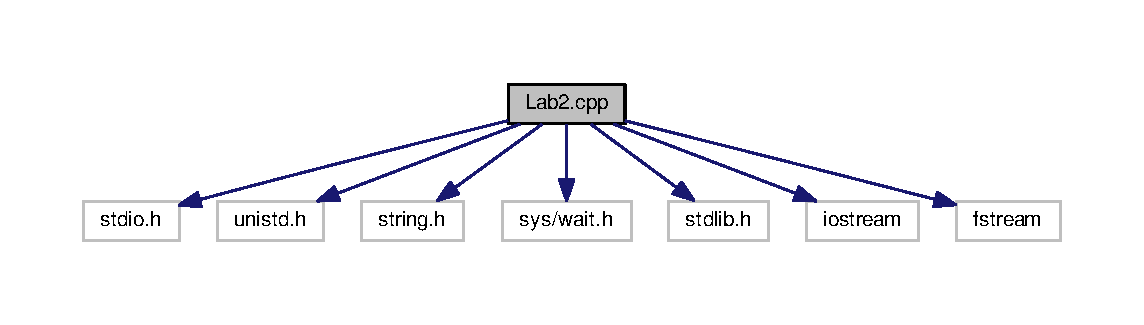
\includegraphics[width=350pt]{Lab2_8cpp__incl}
\end{center}
\end{figure}
\subsection*{Functions}
\begin{DoxyCompactItemize}
\item 
void \hyperlink{Lab2_8cpp_ab2511fed673cd92bb6bbdc5666d7094f}{execute} (char cmdline\mbox{[}$\,$\mbox{]})
\item 
int \hyperlink{Lab2_8cpp_a0ddf1224851353fc92bfbff6f499fa97}{main} (int argc, char $\ast$argv\mbox{[}$\,$\mbox{]})
\end{DoxyCompactItemize}
\subsection*{Variables}
\begin{DoxyCompactItemize}
\item 
const int \hyperlink{Lab2_8cpp_a323c4099d6ea7f155d234fe58b42cfbf}{M\+A\+X\+\_\+\+L\+I\+N\+E\+\_\+\+L\+EN} =1024
\item 
const int \hyperlink{Lab2_8cpp_abf54c72fb5d7d3d82c94537400a0d688}{W\+O\+R\+D\+\_\+\+L\+EN} =51
\item 
const int \hyperlink{Lab2_8cpp_ae021f3fa9060f6386cc3cc6f83430304}{M\+A\+X\+\_\+\+W\+O\+R\+D\+\_\+\+N\+UM} =20
\end{DoxyCompactItemize}


\subsection{Function Documentation}
\index{Lab2.\+cpp@{Lab2.\+cpp}!execute@{execute}}
\index{execute@{execute}!Lab2.\+cpp@{Lab2.\+cpp}}
\subsubsection[{\texorpdfstring{execute(char cmdline[])}{execute(char cmdline[])}}]{\setlength{\rightskip}{0pt plus 5cm}void execute (
\begin{DoxyParamCaption}
\item[{char}]{cmdline\mbox{[}$\,$\mbox{]}}
\end{DoxyParamCaption}
)}\hypertarget{Lab2_8cpp_ab2511fed673cd92bb6bbdc5666d7094f}{}\label{Lab2_8cpp_ab2511fed673cd92bb6bbdc5666d7094f}

\begin{DoxyCode}
65 \{
66    pid\_t pid;
67    \textcolor{keywordtype}{bool} background = \textcolor{keyword}{false};
68    \textcolor{keywordtype}{char} *Word[\hyperlink{Lab2_8cpp_ae021f3fa9060f6386cc3cc6f83430304}{MAX\_WORD\_NUM}]; \textcolor{comment}{//an array of pointer to char...                                  
                                                                                                                  
       }
69 
70    \textcolor{comment}{/*TODO: break cmd lines into an array of words,                                                         
                                                                                                       }
71 \textcolor{comment}{        ignoring anything statring crom character # (if any)                                               
                                                                                                       }
72 \textcolor{comment}{        You can assume different words (command line arguments) are always separated by spaces             
                                                                                                       }
73 \textcolor{comment}{        (you can use function strlen (cmdline) to get the length of a C string...)                         
                                                                                                       }
74 \textcolor{comment}{        You need to split the cmdline into multiple words, each word is an argument                        
                                                                                                       }
75 \textcolor{comment}{        1) replace space by \(\backslash\)0 (terminating character)                                                     
                                                                                                       }
76 \textcolor{comment}{        2) use Word[0] to point to the first char of the first word                                        
                                                                                                       }
77 \textcolor{comment}{           use Word[1] to point to the cirst char of the second word                                       
                                                                                                       }
78 \textcolor{comment}{           use NULL to indicate the end of Word array */}
79 
80    Word[0] = &(cmdline[0]);
81    \textcolor{keywordtype}{int} length = strlen(cmdline);
82    \textcolor{keywordtype}{int} i = 1;
83    \textcolor{keywordflow}{for}(\textcolor{keywordtype}{int} k=0; k<length; k++)
84    \{
85       \textcolor{keywordflow}{if}(cmdline[k] != \textcolor{charliteral}{'#'}) \textcolor{comment}{//ignores comments                                                             
                                                                                                       }
86       \{
87          \textcolor{keywordflow}{if}(cmdline[k] == \textcolor{charliteral}{' '})
88          \{
89             cmdline[k] = \textcolor{charliteral}{'\(\backslash\)0'};
90             \textcolor{keywordflow}{if}(cmdline[k+1] != \textcolor{charliteral}{'#'}) \textcolor{comment}{//ignores comments                                                     
                                                                                                       }
91                Word[i] = &(cmdline[k+1]);
92             i++;
93          \}
94       \}
95    \}
96    \textcolor{comment}{//prepares for if the command is done in the background or not                                          
                                                                                                       }
97    \textcolor{keywordflow}{if}(*Word[i-1] == \textcolor{charliteral}{'&'})
98    \{
99       Word[i-1] = NULL;
100       background = \textcolor{keyword}{true};
101    \}
102    \textcolor{keywordflow}{else}
103       Word[i] = NULL;
104 
105    \textcolor{keywordflow}{if}(!strcmp (cmdline, \textcolor{stringliteral}{"exit"}))
106       exit(0);
107    \textcolor{comment}{/*create a child process*/}
108    pid = fork();
109    \textcolor{keywordflow}{if}(pid < 0)
110    \{
111       fprintf(stderr, \textcolor{stringliteral}{"Fork Failed"});
112       exit(-1);
113    \}
114    \textcolor{keywordflow}{else} \textcolor{keywordflow}{if}(pid == 0)
115    \{
116       \textcolor{comment}{//Todo: checking return value of execvp...                                                           
                                                                                                       }
117       execvp(Word[0], Word);
118 
119       \textcolor{comment}{//If we are here, that menas execvp fails...}
120       cout << \textcolor{stringliteral}{"Command not found\(\backslash\)n"};
121       exit(1);
122    \}
123    \textcolor{keywordflow}{else}
124    \{
125       \textcolor{keywordflow}{if}(!background)
126       \{
127          \textcolor{comment}{//parent will wait for the child to complete                                                      
                                                                                                       }
128          wait(NULL);
129       \}
130    \}
131 \}
\end{DoxyCode}
\index{Lab2.\+cpp@{Lab2.\+cpp}!main@{main}}
\index{main@{main}!Lab2.\+cpp@{Lab2.\+cpp}}
\subsubsection[{\texorpdfstring{main(int argc, char $\ast$argv[])}{main(int argc, char *argv[])}}]{\setlength{\rightskip}{0pt plus 5cm}int main (
\begin{DoxyParamCaption}
\item[{int}]{argc, }
\item[{char $\ast$}]{argv\mbox{[}$\,$\mbox{]}}
\end{DoxyParamCaption}
)}\hypertarget{Lab2_8cpp_a0ddf1224851353fc92bfbff6f499fa97}{}\label{Lab2_8cpp_a0ddf1224851353fc92bfbff6f499fa97}

\begin{DoxyCode}
21 \{
22    \textcolor{keywordtype}{char} *pwd, *host, *usr;
23    \textcolor{keywordtype}{char} cmdline[\hyperlink{Lab2_8cpp_a323c4099d6ea7f155d234fe58b42cfbf}{MAX\_LINE\_LEN}];
24    ifstream scriptFile;
25 
26    \textcolor{comment}{//Calling getenv to find the current values of environment variables                                    
                                                                                                       }
27    pwd = getenv(\textcolor{stringliteral}{"PWD"});
28    host = getenv(\textcolor{stringliteral}{"HOSTNAME"});
29    usr = getenv(\textcolor{stringliteral}{"USER"});
30 
31    \textcolor{comment}{//error if there are more than two arguments                                                            
                                                                                                       }
32    \textcolor{keywordflow}{if}(argc > 2)
33    \{
34       cout << \textcolor{stringliteral}{"ERROR: too many arguments\(\backslash\)n"};
35       exit(1);
36    \}
37    \textcolor{comment}{//read from file if there are two arguments                                                             
                                                                                                       }
38    \textcolor{keywordflow}{if}(argc == 2)
39    \{
40       scriptFile.open(argv[1]);
41       \textcolor{keywordflow}{if}(!scriptFile.is\_open())
42          \_exit(1);
43       \textcolor{keywordflow}{while}(scriptFile.good())
44       \{
45          scriptFile.getline(cmdline, 256);
46          \textcolor{keywordflow}{while}(cmdline[0] == \textcolor{charliteral}{'#'}) \textcolor{comment}{//ignores the comments                                                   
                                                                                                       }
47             scriptFile.getline(cmdline, 256);
48          \textcolor{keywordflow}{if}(scriptFile.good())
49             \hyperlink{Lab2_8cpp_ab2511fed673cd92bb6bbdc5666d7094f}{execute}(cmdline);
50       \}
51       scriptFile.close();
52    \}
53    \textcolor{comment}{//read from terminal if there is only 1 argument                                                        
                                                                                                       }
54    \textcolor{keywordflow}{if}(argc == 1)
55    \{
56       \textcolor{keywordflow}{while}(1)
57       \{
58          cout << \textcolor{stringliteral}{"["} << usr << \textcolor{stringliteral}{"@"} << host << \textcolor{stringliteral}{" "} << pwd << \textcolor{stringliteral}{"]$"};
59          cin.getline(cmdline, 256);
60          \hyperlink{Lab2_8cpp_ab2511fed673cd92bb6bbdc5666d7094f}{execute}(cmdline);
61       \}
62    \}
63 \}
\end{DoxyCode}


Here is the call graph for this function\+:
\nopagebreak
\begin{figure}[H]
\begin{center}
\leavevmode
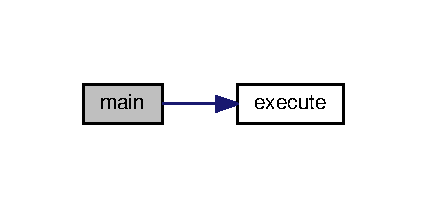
\includegraphics[width=205pt]{Lab2_8cpp_a0ddf1224851353fc92bfbff6f499fa97_cgraph}
\end{center}
\end{figure}




\subsection{Variable Documentation}
\index{Lab2.\+cpp@{Lab2.\+cpp}!M\+A\+X\+\_\+\+L\+I\+N\+E\+\_\+\+L\+EN@{M\+A\+X\+\_\+\+L\+I\+N\+E\+\_\+\+L\+EN}}
\index{M\+A\+X\+\_\+\+L\+I\+N\+E\+\_\+\+L\+EN@{M\+A\+X\+\_\+\+L\+I\+N\+E\+\_\+\+L\+EN}!Lab2.\+cpp@{Lab2.\+cpp}}
\subsubsection[{\texorpdfstring{M\+A\+X\+\_\+\+L\+I\+N\+E\+\_\+\+L\+EN}{MAX_LINE_LEN}}]{\setlength{\rightskip}{0pt plus 5cm}const int M\+A\+X\+\_\+\+L\+I\+N\+E\+\_\+\+L\+EN =1024}\hypertarget{Lab2_8cpp_a323c4099d6ea7f155d234fe58b42cfbf}{}\label{Lab2_8cpp_a323c4099d6ea7f155d234fe58b42cfbf}
\index{Lab2.\+cpp@{Lab2.\+cpp}!M\+A\+X\+\_\+\+W\+O\+R\+D\+\_\+\+N\+UM@{M\+A\+X\+\_\+\+W\+O\+R\+D\+\_\+\+N\+UM}}
\index{M\+A\+X\+\_\+\+W\+O\+R\+D\+\_\+\+N\+UM@{M\+A\+X\+\_\+\+W\+O\+R\+D\+\_\+\+N\+UM}!Lab2.\+cpp@{Lab2.\+cpp}}
\subsubsection[{\texorpdfstring{M\+A\+X\+\_\+\+W\+O\+R\+D\+\_\+\+N\+UM}{MAX_WORD_NUM}}]{\setlength{\rightskip}{0pt plus 5cm}const int M\+A\+X\+\_\+\+W\+O\+R\+D\+\_\+\+N\+UM =20}\hypertarget{Lab2_8cpp_ae021f3fa9060f6386cc3cc6f83430304}{}\label{Lab2_8cpp_ae021f3fa9060f6386cc3cc6f83430304}
\index{Lab2.\+cpp@{Lab2.\+cpp}!W\+O\+R\+D\+\_\+\+L\+EN@{W\+O\+R\+D\+\_\+\+L\+EN}}
\index{W\+O\+R\+D\+\_\+\+L\+EN@{W\+O\+R\+D\+\_\+\+L\+EN}!Lab2.\+cpp@{Lab2.\+cpp}}
\subsubsection[{\texorpdfstring{W\+O\+R\+D\+\_\+\+L\+EN}{WORD_LEN}}]{\setlength{\rightskip}{0pt plus 5cm}const int W\+O\+R\+D\+\_\+\+L\+EN =51}\hypertarget{Lab2_8cpp_abf54c72fb5d7d3d82c94537400a0d688}{}\label{Lab2_8cpp_abf54c72fb5d7d3d82c94537400a0d688}

%--- End generated contents ---

% Index
\backmatter
\newpage
\phantomsection
\clearemptydoublepage
\addcontentsline{toc}{chapter}{Index}
\printindex

\end{document}
